
\clearpage
\section{Address List}
\label{bkm:Ref443738751}
In the address list, all persons (users) and companies (participants) registered in CUBE PA are displayed in a simple way. Using the filter function, the desired entries can quickly be found.

\vspace{\baselineskip}

The following properties should be taken into account when using the address list:

% \liststyleWWviiiNumxiii
\begin{itemize}
\item
An authorized CUBE PA user can add new persons and companies to the address list or edit existing entries.

\item
Persons who have been added this way are automatically available in all person selection fields (e.g., actions). However, these newly registered persons cannot log in to CUBE PA. If this is desired, the administrator can help, or contact with CUBE PA Support should be made 
(see chapter \ref{bkm:Ref443502661}).

\item
If a person is assigned to a company, the company address automatically appears in the address list. If this is not desired e.g. due to different company locations, a specific address can be added in 
the editing window of the person.

\item
For persons who can actively log in to CUBE PA, membership to a company can only be changed by the administrator for security reasons (access rights). Please report such mutations to the administrator, resp. the CUBE PA support (see chapter \ref{bkm:Ref443502661}).

\item
Company entries that are added to the address list are not automatically available as tenderers or clients in procurement management. If companies are also to be displayed in procurement management, this must be accordingly configured by the administrator.
\end{itemize}

\pagebreak
\subsection{Finding persons or companies in the address list}

\begin{wrapfigure}[2]{l}{6.5cm}   % [x] Wie manche Zeile soll sich um die Grafik "brechen"
  \vspace{-35pt}      % Grundwert war 20; mit 30 schön oben beim Text ausgerichtet
  \begin{center}
    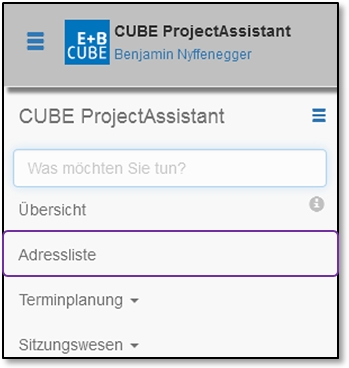
\includegraphics[width=1\linewidth]{../chapters/03_Adressliste/pictures/3-1_Menu_Adressliste.jpg}
  \end{center}
  \vspace{-20pt}
  \caption{Using the address list}
  \vspace{-10pt}
\end{wrapfigure}

Select the field 'Address List' in the menu on the left.

\vspace{7cm}

A list with all the addresses of persons and companies entered in CUBE PA is displayed:

\begin{figure}[H]
\center{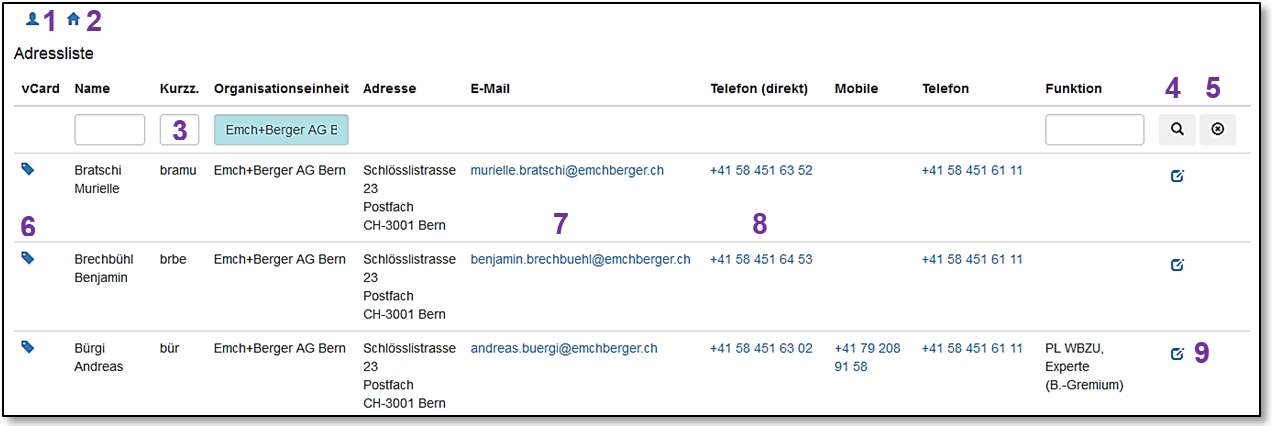
\includegraphics[width=1\linewidth]{../chapters/03_Adressliste/pictures/3-1_Adressliste_Uebersicht.jpg}}
\caption{Overview of the address list}
% \label{fig:speciation}
\end{figure}

In the top left you can add new persons 
\includegraphics[height=12pt]{/Icons/Person.jpg} or organisational units 
\includegraphics[height=12pt]{/Icons/Haus.jpg}. Take the properties listed at the beginning of the chapter into consideration (Chapter \ref{bkm:Ref443738751}). \newline
To search / filter through the entries, two fields can be used. Enter a search term in the field 'Name' or 'Organisational Unit' \col{(3)} and click on the magnifying glass (search) symbol 
\includegraphics[height=12pt]{/Icons/Lupe_kl.jpg} \col{(4)} or press the 'Enter' key. All found entries will be shown. Click the cross (reset search) \col{(5)} to reset all the filter settings. \newline
You can download a vCard (Address card, for example for Outlook). Click on the vCard symbol 
\includegraphics[height=12pt]{/Icons/vCard.jpg} \col{6)}. You will be asked if you want to open or 
save the vCard.\newline
Click on the e-mail address \col{(7)} to send an e-mail to the selected person. Click on the telephone number \col{(8)} to call the person e.g. using Skype (depending on the installation).\newline
Click the editing symbol 
\includegraphics[height=12pt]{/Icons/Bearbeiten.jpg} \col{(9)} to modify the entry of a person or an organisational unit. However, you need to have the required access rights to do so. Click on the pencil symbol 
\includegraphics[height=12pt]{/Icons/Stift.jpg} \col{(10)} to go directly to the user settings (in the user management menu). You also need the required access rights to make changes.

\subsection{Adding new persons or companies to the address list}
Authorized users can add new persons or companies to the address list or modify existing entries:

\vspace{\baselineskip}

\begin{tabular}{cc} %{cl}
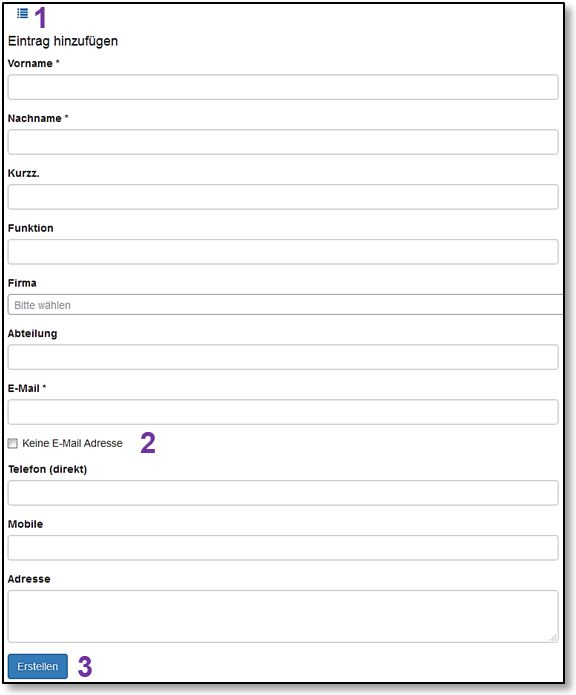
\includegraphics[width=0.49\textwidth]{32_Personeneintraege.jpg} & 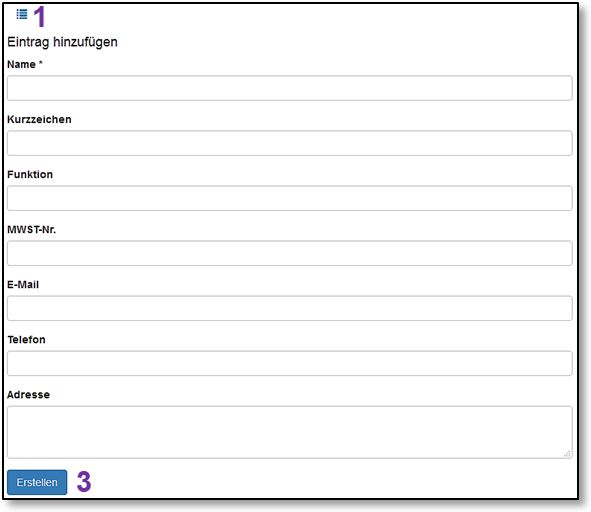
\includegraphics[width=0.49\textwidth]{32_Firmeneintraege.jpg} \\
Person and company entries \\
\end{tabular}

% \begin{figure} 
%      \subfigure{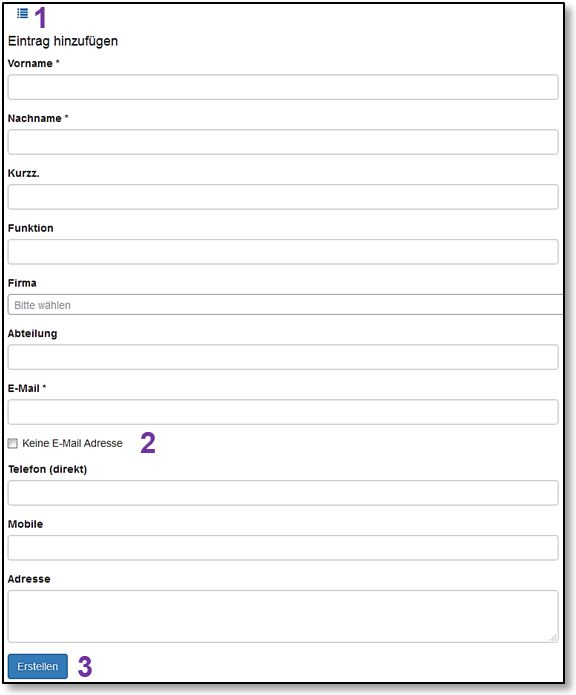
\includegraphics[width=0.49\textwidth]{32_Personeneintraege.jpg}} 
%      \subfigure{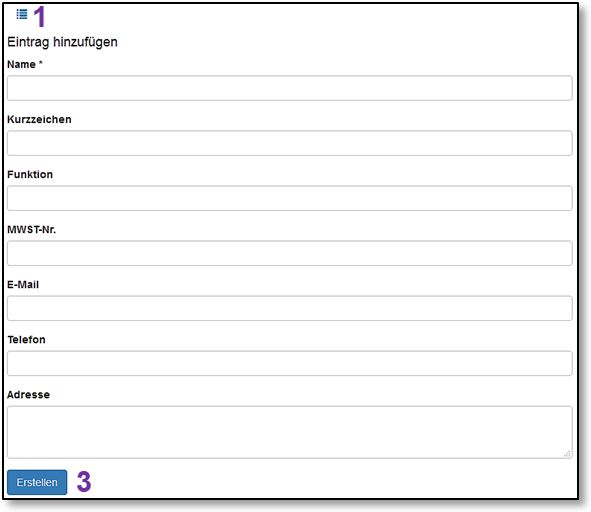
\includegraphics[width=0.49\textwidth]{32_Firmeneintraege.jpg}} 
% \caption{Die verschiedenen Eingabemasken der Adressliste} 
% \end{figure}

\vspace{\baselineskip}
All fields marked with a * are mandatory fields and must be filled out. If no e-mail address is to be entered, the e-mail field can be bypassed and left blank by checking the 'No e-mail' check-box. After entering the desired / known data, the data record can be saved by clicking the 'Create' button \col{(3)} and is made available in the address list. If you click the editing symbol 
\includegraphics[height=12pt]{/Icons/Bearbeiten.jpg} of an existing entry, the same form (see above) will be opened. All already stored data is available in the corresponding fields and can be edited. As noted at the beginning of the chapter, the company membership of a person cannot be changed, resp. can only be changed via the administrator, for security reasons (access rights).\newline
Click on the list symbol 
\includegraphics[height=12pt]{/Icons/Listensymbol_zurueck.jpg} \col{(1)} to return to the address list.
